\chapter[Procesos atmosf\'ericos]{Fisicoqu\'{\i}mica en procesos atmosf\'ericos}

Los procesos fisicoquímicos en la atmósfera son fundamentales para comprender la dinámica de los contaminantes, la formación de fenómenos ambientales y el equilibrio natural de los sistemas terrestres. Este capítulo explora los principios que gobiernan las interacciones entre fases, la termodinámica atmosférica y los mecanismos que regulan la transformación de sustancias en la troposfera y estratosfera.

En la Sección~\ref{solub}, se analiza la \textbf{solubilidad} como eje central de los equilibrios aire-agua, clave para entender la partición de contaminantes entre fases gaseosas y líquidas. Se aborda el equilibrio acuoso (\ref{eacuoso}) y la solubilidad de gases en agua (\ref{sgases}), procesos que determinan la concentración atmosférica de especies como el \ce{CO2} y \ce{SO2}, y su impacto en fenómenos como la lluvia ácida.

La Sección~\ref{llacd} profundiza en la \textbf{lluvia ácida}, desde su contexto histórico (\ref{hllacd}) hasta sus mecanismos de formación, vinculando la química de óxidos de azufre y nitrógeno con los equilibrios ácido-base en nubes y precipitaciones. Este fenómeno ejemplifica cómo los procesos de solubilidad y cinética química (Sección~\ref{vreac}) interactúan a escala global.

Las bases termodinámicas (Sección ~\ref{tatm}) y el comportamiento del \textbf{aire húmedo vs. aire seco} (\ref{ahas}) se exploran mediante conceptos como la flotabilidad de parcelas aéreas (\ref{flopa}) y su aceleración (\ref{acpa}), esenciales para modelar la estabilidad atmosférica y el transporte vertical de contaminantes.

En las Secciones~\ref{cineq}  a \ref{fqm}, se integran herramientas cuantitativas para caracterizar:
\begin{itemize}
    \item Velocidades de reacción (\ref{vreac}) y su dependencia de parámetros cinéticos
    \item Tiempos de vida media (\ref{TVDM}) y residencia atmosférica (\ref{tdres})
    \item Procesos fotoquímicos (\ref{fqm}) activados por radiación solar
\end{itemize}

Finalmente, la Sección~\ref{vis2} aborda la \textbf{visibilidad} como aplicación práctica de estos principios, analizando los mecanismos de dispersión lumínica (\ref{mddis}) y su relación con aerosoles submicrométricos. Los ejercicios al final del capítulo permiten aplicar estos conceptos a casos reales, desde el cálculo de equilibrios hasta la estimación de tiempos de degradación de contaminantes.

Este enfoque multiescala conecta fenómenos moleculares (equilibrios de fase) con impactos globales (acidificación), destacando cómo la fisicoquímica atmosférica explica y predice desafíos ambientales críticos..  

 \section{Solubilidad}\index{solubilidad}
 \label{solub}
 
Una soluci\'on es una mezcla homog\'enea de sustancias. Cuando el az\'ucar se disuelve en agua, una mezcla homog\'enea o soluci\'on se forma. El componente que presenta la mayor cantidad en la mezcla determina la fase o el estado (s\'olido, l\'{\i}quido, o gas) de la soluci\'on es el \emph{\gloss[word]{solvente}}.\index{solvente} El otro componente es conocido como \emph{\gloss[word]{soluto}}.\index{soluto} Si se emplea agua como solvente, se dice que la soluci\'on es acuosa (ac).\index{solucion@soluci\'on!acuosa} Ejemplos de soluciones comunes se muestran en el \textbf{Cuadro~\ref{soluciones}}.

 \begin{table}[hbt]
\caption{ Ejemplos de soluciones}
{\footnotesize
 \begin{tabular}{llll}
Soluci\'on & Estado de la  & Estado del & Estado del(os) \\
           & Soluci\'on    & Solvente   & Soluto(s) \\\hline
Atm\'osfera terrestre & Gas & Gas \ce{N2} & Gas-\ce{O2}, Ar, \ce{CO2}\\
Agua de Oceano & L\'{\i}quido & L\'{\i}quido-\ce{H2O} & S\'olido-sales-NaCl\\
               &              &                 & gas--\ce{O2}, \ce{CO2}\\
Joyer\'{\i}a de oro &     S\'olida & S\'olido--Au    & S\'olido--Ag,Cu\\
Agua de acuario&     Liquida  & L\'{\i}quido--\ce{H2O} & Gas--\ce{O2}, \ce{CO2}\\
Di\'oxido de carbono en hielo &S\'olido & S\'olido--hielo &Gas--\ce{CO2}\\\hline
\end{tabular}}
\label{soluciones}
\end{table}

\subsection{Equilibrio acuoso}
\index{equilibrio!acuoso}\label{eacuoso}

Hemos revisado con anterioridad los principios b\'asicos del equilibrio qu\'{\i}mico. Ahora aplicaremos estos principios al equilibrio ionico en soluciones acuosas.

Como punto de partida consideremos, ls disoluci\'on del sulfato de plata en agua (\ce{Ag2SO4})
\reaction{Ag2SO4 <=> 2Ag+(ac) + SO4^2-(ac)}
 
La constante de equilibrio para esta reacci\'on es:\\[2pt]

\hskip 3cm $K_{ps} = $ [\ce{Ag+(ac)}]$^2$[\ce{SO4^2-(ac)}] $=$1.4$\times10^{-5}$\\[2pt]

Si C son las moles de sulfato de plata en agua,  C moles de sulfato de plata se disuelven en 1 L de agua para producir 2C moles de i\'on plata (\ce{2Ag+}) y C moles de i\'on sulfato (\ce{SO4^2-}). As\'{\i}, $K_{ps}=$1.4$\times10^{-5} = C^3$ o $C=$ 0.0241 M. Por lo tanto, s\'olo 0.0241 moles de sulfato de plata se disuelven en 1L de agua.

Como $K_{ps}$ es el producto de las concentraciones de los iones, se le llama \emph{constante producto de solubilidad} (por eso el sub\'{\i}ndice ''ps``). El producto de solubilidad se usa generalmente para sustancia con bajas solubilidades. \index{producto!de solubilidad}

Los productos de solubilidad muy bajos se miden el\'ectricamente y esos valores se reportan en las tablas. Generalmente se listan los productos de solubilidad de sustancias poco solubles o parcialmente insolubles. Si la $K_{ps}$ es muy baja, se considera una sustancia \emph{insoluble}\index{insoluble} (en agua). En el caso de sustancias con solubilidad moderada o alta (como el NaCl o NaOH), no es \'util el empleo de los productos de solubilidad. Por que en lugar de definir  la constante de equilibrio en t\'erminos de concentraci\'on tendremos que definirla en t\'erminos de la \emph{actividad} de las sustancias.\index{actividad}

\begin{table}[hbt]
\caption{Solubilidades en agua de algunos compuestos}
\hskip 0.5in\begin{tabular}{lll}\hline
Iones Negativos & Iones Positivos & Solubilidad\\
(aniones) & (cationes) & \\\hline
Todos               & \ce{Li+}, \ce{Na+}, K$^+$, Rb$^+$, Cs$^+$, Fr$^+$ & Soluble\\
Todos               & \ce{H+}             & Soluble\\
Todos               & \ce{NH4+} (amonio)  & Soluble\\
\ce{NO3-} nitrato   & Todos               & Soluble \\ 
\ce{CH3COO-} acetato& Todos               & Soluble\\
\ce{SO4^2-} sulfato & \ce{Ba^2+}, \ce{Sr^2+}, \ce{Pb^2+},\ce{Ca^2+} & Poco soluble\\
                    & Todos los dem\'as   & Soluble\\\hline 
\end{tabular}
\end{table}

 \subsection{Solubilidad de gases en agua}
\label{sgases}

 Algebr\'aicamente, podemos expresar las propiedades de la soluci\'on  diluida ideal mediante las siguientes ecuaciones:
\begin{eqnarray}
 p_1&= &x_1p_1^\circ\label{raoult}\\
 p_j&=& K_jx_j
 \label{henry}
 \end{eqnarray}
 
 Donde el sub\'{\i}ndice denota cualquiera de los solutos y el sub\'{\i}ndice uno denota el solvente. Todas las soluciones reales se aproximan al comportamiento descrito por las ecuaciones~\ref{raoult} y \ref{henry}, siempre y cuando  la soluci\'on est\'e suficientemente dilu\'{\i}da. Lo mismo es v\'alido si est\'an presentes varios solutos, pero la soluci\'on debe estar diluida en todos; cada soluto tiene un valor diferente de $K_j$.
 
 La Ley de \gloss[Word]{henry}, ecuaci\'on \ref{henry},  \index{Henry@\textbf{Henry}!ley de} relaciona la presi\'on parcial del soluto en la fase vapor con la fracci\'on molar del soluto en la soluci\'on a temperatura constante. Enfocando la relaci\'on desde otro punto de vista, la ley de Henry relaciona la fracci\'on molar en el equilibrio, solubilidad de \emph{j} en la soluci\'on, con la presi\'on parcial de \emph{j} en el vapor:
 
 \begin{equation}
x_j=\frac{1}{K_j}p_j
\label{henry2}
\end{equation}

La ecuaci\'on~\ref{henry2} expresa que la solubilidad $x_j$ de un constituyente vol\'atil es proporcional a la presi\'on parcial del mismo en la fase gaseosa en equilibrio con el l\'{\i}quido. La ecuaci\'on~\ref{henry2} se emplea para correlacionar los datos de solubilidad de gases en l\'{\i}quidos. Si el solvente y el gas no reaccionan qu\'{\i}micamente, la solubilidad de gases en l\'{\i}quidos es peque\~na, por lo general, de modo que se cumple la condici\'on de diluci\'on. 

\section{Lluvia \'acida}
\index{lluvia!acida@\'acida}\label{llacd}

\subsection{Historia de la lluvia \'acida}
\label{hllacd}
En el siglo XIX, la gente comenz\'o a darse cuenta de que la suciedad expulsada por las chimeneas de las viviendas y f\'abricas estaba ocasionando la contaminaci\'on de la lluvia. En \'epocas anteriores, la gente se hab\'{\i}a quejado del desagradable ambiente generado por el humo de las chimeneas. La lluvia \'acida puede producirse de forma natural. Los volcanes, las turberas y las plantas en descomposici\'on desprenden di\'oxido de azufre.

\begin{tabular}{cl}
1692 & Rob Boyle\\
     & En su libro ``General History of the Air''\\
     & incluye discusiones de ``Esp\'{\i}ritus nitrosos o sulfuros salinos''\\
1872 & Robert Angus Smith\\
     & En el libro ``The beginning of Chemical Climatology'' describi\'o \\
     & la importancia de las fuentes de combusti\'on de carb\'on en la precipi-\\
     & ta\-ci\-\'on m\'etodos de muestreo, da\~no a plantas y materiales.
\end{tabular}

La absorci\'on de \ce{CO2} en el agua de lluvia cambia el $p$H.  Para observar esto podemos aplicar los conocimientos anteriores. La solubilidad del \ce{CO2} en agua viene dada por:

\reaction{CO2_{(g)} + H2O <=> H2CO3_{(ac)}}

Para el equilibrio del \ce{CO2} con el \ce{H2O}, empleamos la constante de Henry ($H$)\index{Henry@\textbf{Henry}!constante} y la presi\'on parcial del \ce{CO2} ($P_{CO_2}$) y obtenemos la concentraci\'on del \'acido carb\'onico (\ce{H2CO3}):
\begin{equation}
[\ce{CO2.H2O}] =P_{\ce{CO2}}H \label{eq1}
\end{equation}

Como hemos visto el \'acido carb\'onico es un \'acido \emph{polipr\'otico}:

\reaction{H2CO3_{(ac)} + H2O_{(l)} <=> HCO3^-_{(ac)} + H3O^+_{(ac)}}
\reaction{HCO3^-_{(ac)} + H2O_{(l)} <=> CO3^{-2}_{(ac)} + H3O^+_{(ac)}}
con las constantes de disociaci\'on  a 25\celsius de $K_a=4.2\times10^{-7}$ y $K_{a2}=5.0\times10^{-11}$. Por lo tanto:
\begin{eqnarray}
\frac{[\ce{H3O+}][\ce{HCO3^-_{(ac)}}]}{[\ce{H2CO3_{(ac)}}]}&=K_{a1}=&4.2\times10^{-7}\label{ec1}\\
\frac{[\ce{H3O+_{(ac)}}][\ce{CO3^{-2}_{(ac)}}]}{[\ce{HCO3^-_{(ac)}}]}&=K_{a2}=&5.0\times10^{-11}\label{ec2}
\end{eqnarray}

Ahora calculemos la concentraci\'on de \ce{H3O+(ac)}, \ce{H2CO3(ac)}, \ce{HCO3^-(ac)}, \\  \ce{OH-}(ac), y \ce{CO3^{-2}(ac)} cuando el \ce{CO2} de la atm\'osfera se disuelve en agua pura de lluvia, dado que la solubilidad del \ce{CO2} en agua es $1.0\times10^{-5}$M a 25$^\circ C$ y 1 atm.  Como se tienen cinco inc\'ognitas se requieren de cinco ecuaciones  para resolver este problema y hasta hora tenemos dos ecuaciones~\ref{ec1} y \ref{ec2}. Las otras tres ecuaciones son dadas por la constante del producto i\'onico del agua ($K_w$):
\begin{equation}
[\ce{H3O+_{(ac)}}][\ce{OH-_{(ac)}}]=K_w=1.0\times10^{-14} \label{ec3}
\end{equation}
del balance de masa
\begin{equation}
[\ce{H2CO3}]\textrm{\footnotesize inicial} = 1.0\times10^{-5} M =
[\ce{H2CO3_{(ac)}}] +[\ce{HCO3-}]+[\ce{CO3^{-2}}]
\label{ec4}
\end{equation}
y la reacci\'on de balanceo de cargas:$$[\ce{H3O+}]=\sum n[x^{N-}]$$
\begin{equation}
[\ce{H3O+(ac)}]= [\ce{HCO3^-(ac)}] +2[\ce{CO3^{-2}(ac)}]+[\ce{OH^-(ac)}]
\label{ec5}
\end{equation}

Donde $1.0\times10^{-5}M$ en la Ec.~\ref{ec4} sigue el hecho de que por cada mol de \ce{CO2} disuelto en agua una mol  de \ce{H2CO3} se forma  (\ce{CO2 + H2O <=> H2CO3}) y el coeficiente 2 en la Ec.~\ref{ec5}  permite dos unidades negativas de carga por cada \ce{CO3^2-}.


Despejando el \ce{HCO3-} de la ecuaci\'on~\ref{ec1}  y sustituyendo el [\ce{CO2.H2O}] a partir de la ecuaci\'on~\ref{eq1} tenemos:

\begin{equation}
[\ce{HCO3-}]=\frac{k_1[\ce{CO2.H2O}]}{[\ce{H+}]}  = \frac{k_1H P_{\ce{CO2}}}{[\ce{H+}]}
\label{ec6}
\end{equation}

De la ecuaci\'on~\ref{ec2} despejamos el \ce{CO3^{-2}} 

\begin{equation}
[\ce{CO3^{-2}}]= \frac{k_2[\ce{HCO3-}]}{[\ce{H+}]}= \frac{k_1k_2HP_{\ce{CO2}}}{[\ce{H+}]^2}
\label{ec7}
\end{equation}

Se desea saber cual es el p$H$ del agua en equilibrio en la atm\'osfera donde se tiene  una  presi\'on parcial de \ce{CO2} ($P_{\ce{CO2}}$), as\'{\i} sustituimos en la ecuaci\'on~\ref{ec5} las ecuaciones \ref{ec6} y \ref{ec7}.

La concentraci\'on del \ce{OH-} la obtenemos de la constante de disociaci\'on del agua $K_w$ y tenemos que,
$K_w = [\ce{H3O+}][\ce{OH-}]$ despejando $[\ce{OH-}]$ de la ecuaci\'on~\ref{ec3} y sustituyendo esto en la ecuaci\'on~\ref{ec5} tenemos:

\begin{equation}
[\ce{H+}]=\frac{k_1H P_{\ce{CO2}}}{[\ce{H+}]} + 2 \frac{k_1k_2HP_{\ce{CO2}}} {[\ce{H+}]^2}+\frac{K_w}{[\ce{H+}]}
\end{equation}

Rearreglando obtenemos:

\begin{equation}
[\ce{H+}]^3 - (K_w +k_1HP_{\ce{CO2}})[\ce{H+}] - 2Hk_1k_2P_{\ce{CO2}}
\end{equation}

para una presi\'on parcial $P_{CO_2} = 380\times10^{-6}$ atm se obtiene a partir de resolver la ecuaci\'on c\'ubica: [\ce{H+}]=10$^{-5.6}$ entonces el p$H$= 5.6
\\

Para el caso del \ce{NH3}
$$\ce{NH3_{ac} <=> NH4^+ + OH^-}$$

Entonces:
\begin{equation*}
H_{\ce{NH3}} =\frac{ [\ce{NH_{3(ac)}}]} { P_{\ce{NH3}}} = 5.8\times10^1\frac{M}{atm}
\end{equation*}

\begin{equation*}
k =\frac {[\ce{NH4^+}][OH^-]} {[\ce{NH_{3(ac)}}]} = 5.6\times10^{-10}
\end{equation*}

\begin{equation*}
\ce{NH4^+} = \frac{k_1H_{\ce{NH3}}P_{\ce{NH3}}\cdot [H^+]} { Kw} 
\end{equation*}

\begin{equation*}
[H^+] + [\ce{NH4+}] = [OH^-] + [\ce{HCO3-}] +2[\ce{CO3^2-}]
\end{equation*}

Para el caso del \ce{SO2}


\begin{equation*}
[\ce{SO2}\cdot\ce{H2O}] = H_{\ce{SO2}} P_{\ce{SO2}}
\end{equation*} 
\begin{equation*}
H_{\ce{SO2}} =\frac{ [\ce{SO2}\cdot\ce{H2O}]} { P_{\ce{SO2}}} = 1.2\frac{\textrm{M}}{\textrm{atm}}
\end{equation*}

\begin{equation*}
k'_1 = \frac{[\ce{H+}][\ce{HSO3^-]}} {[\ce{H2SO3}]} = 1.71\times10^{-2}
\end{equation*}

\begin{equation*}
k'_2 = \frac{[H^+] [\ce{SO3^{2-}}]}{[\ce{HSO3-}]} = 5.98\times10^{-8}
\end{equation*}

\begin{equation*}
[H^+] = [OH^-] + [\ce{HSO3-}] +2[\ce{SO3^{-2}}]
\end{equation*}

Despejando de k$'_1$  el [\ce{HSO3-}], de  k$'_2$  el [\ce{SO3^{-2}}]

\begin{equation*}
[\ce{HSO3-}] =\frac{ k_1[\ce{H2SO3}]} {[H^+]} 
\end{equation*}

\begin{equation*}
[\ce{HSO3-}]= \frac{k_1 H_{\ce{H2SO3}}P_{\ce{H2SO3}}} {[\ce{H+}]}
\end{equation*}

\begin{equation*}
[\ce{SO3^{2-}}] =\frac{k_2[\ce{HSO3-}]} {[\ce{H+}]} 
\end{equation*}

\begin{equation*}
[\ce{SO3^{2-}}]=\frac{k'_1k'_2H_{\ce{H2SO3}}P_{\ce{H2SO}}} {[H^+]}
\end{equation*}

Juntando los tres compuestos obtenemos:

\begin{equation*}
[H^+] + [\ce{NH4+}] = [\ce{OH-}]+[\ce{HCO3-}]+2[\ce{CO3^{2-}}]+[\ce{HSO3-}]+2[\ce{SO^{2-}}]
\end{equation*}

 \begin{equation*}
\begin{split}
[\ce{H+}] + \frac{kH_{\ce{NH3}}P_{\ce{NH3}}}{[\ce{OH-}]} &= [\ce{OH-}] + \frac{k_1H_{\ce{CO2}}P_{\ce{CO2}}}{[\ce{H+}]} +\frac{2k_1k_2H_{\ce{CO2}}P_{\ce{CO2}}}{[\ce{H+}]^2} + \\
&\quad\frac{k'_1H_{\ce{SO2}}P_{\ce{SO2}}} {[\ce{H+}]} + \frac{2k'_1k'_2H_{\ce{SO2}}P_{\ce{SO2}}}{[\ce{H+}]^2}
\end{split}
\end{equation*}

sustituyendo el [\ce{OH-}]  por  $\frac{K_w}{[\ce{H+}]} $ queda: 
 \begin{equation*}
\begin{split}
[H^+] + \frac{kH_{\ce{NH3}}P_{\ce{NH3}}[H^+]}{Kw} &= \frac{Kw}{[H^+]} + \frac{k_1H_{\ce{CO2}}P_{\ce{CO2}}}{[H^+]} +\frac{2k_1k_2H_{\ce{CO2}}P_{\ce{CO2}}}{[H^+]^2} +\\ &\quad\frac{k'_1H_{\ce{SO2}}P_{\ce{SO2}}} {[H^+]} + \frac{2k'_1k'_2H_{\ce{SO2}}P_{\ce{SO2}}}{[H^+]^2}
\end{split}
\end{equation*}

\section{Termodin\'amica en la atm\'osfera.}
\label{tatm}

Si se desea conocer en la atm\'osfera si  el aire caliente se desplaza hacia arriba o hacia abajo, o identificar 
?`cu\'al ser\'{\i}a el cambio en la temperatura con la elevaci\'on?, y ?`c\'omo se puede describir matem\'aticamente esto?. Se puede aplicar  la primera ley de la termodin\'amica y la ley general de los gases ideales de la siguiente manera:
\begin{equation}
\mathrm{d}Q =Cp\,\mathrm{d}T -V\,\mathrm{d}P
\end{equation}
Donde:

{\small \begin{tabular}{r@{ -- }l}
$\mathrm{d}Q$ & calor adicionado a la parcela de aire (\joule/\kilogram)\\
$Cp$ & calor espec\'{\i}fico a presi\'on constante\footnote{capacidad t\'ermica espec\'{\i}fica o capacidad cal\'orica espec\'{\i}fica} (\joule/\kilogram\kelvin)\\
$\mathrm{d}T$ & cambio en la temperatura (\kelvin)\\
$V$  & volumen de una unidad de masa (\metre$^3$/\kilogram)\\
$\mathrm{d}P$ & incremento en la presi\'on de la parcela (\pascal)\\
\end{tabular}}
\begin{enumerate}
\item Se considera que la parcela no intercambia calor con los alrededores (\textit{adiab\'atica}) y entonces tenemos que $\mathrm{d}Q =0$, rearreglando la ecuaci\'on anterior nos da:
\begin{equation}
\frac{\mathrm{d}T}{\mathrm{d}P}=\frac{V}{Cp}
\label{equ:1}
\end{equation}
\item Una forma de relacionar  el cambio de temperatura con la elevaci\'on en una atm\'osfera hisdrost\'atica es considerando una parcela de  aire cuyo espesor es $\mathrm{d}z$ y con un \'area $A$,  de esta forma su peso es $g\rho A\,\mathrm{d}z$.
\begin{center}
\begin{picture}(50,35)
\put (5,5){\line(2,1){7}} %Linea inf derecha
\put(12,8.5){\line(1,0){20}}% linea inf de atras
\put(12,8.5){\line(0,1){25}}
\thicklines
\put(5,30){\line(1,0){20}\line(2,1){7}} %Lineas superiores
\put(5,30){\line(2,1){7}}
\put(12,33.5){\line(1,0){20}} 
\put (5,5){\line(1,0){20}\line(2,1){7}} % Lineas Inferiores
\multiput(5,5)(20,0){2}{\line(0,1){25}}
\put(32,8.5){\line(0,1){25}}
% Flecha y texto izquierdo
\put(3,19){\vector(0,1){11}}
\put(3,15){\vector(0,-1){10}}
\put(0,16){$\mathrm{d}z$}
% Parte derecha
\put(34,8){{\footnotesize $P(z)$}}
\put(34,32){\footnotesize $P(z+\mathrm{d}z)$}
% Parte inferior
\put(15,6){{\scriptsize $A$}}
\end{picture}
\end{center}
As\'{\i}  la presi\'on en la parte inferior de la parcela ($P_{(z)}$) incluye la presi\'on de la parte superior de la parcela ($P_{(z+\mathrm{d}z)}$), m\'as la presi\'on debida al peso de la parcela ($\frac{g \rho A\, \mathrm{d}z}{A}$). Con base en lo anterior  tenemos:
\begin{equation}
P(z) = P(z+\mathrm{d}z) +\frac{g \rho A\,\mathrm{d}z}{A}
\end{equation}
\'o
\begin{equation}
dP =P(z+\mathrm{d}z) - P(z) = -g\rho\, \mathrm{d}z
\end{equation}
simplificando y factorizando tenemos la ecuaci\'on hidrost\'atica que se representa:
\begin{equation}
\frac{dP}{\mathrm{d}z}= -g\rho
\label{equ:2}
\end{equation}
\item Aplicando la regla de la cadena para  la ecuaci\'on \ref{equ:1}  y la   \ref{equ:2}, 
%\begin{equation}
%\frac{dT}{dP} = \frac{V}{Cp}
%\end{equation}
con el objeto de obtener $\frac{\mathrm{d}T}{\mathrm{d}z}$ nos da,
\begin{equation}
\frac{\mathrm{d}T}{\mathrm{d}z}=\frac{\mathrm{d}T}{\mathrm{d}P}\frac{\mathrm{d}P}{\mathrm{d}z} =\frac{V}{Cp}(-g\rho)
\end{equation}
Conociendo que volumen por unidad de masa ($V$) y la densidad por unidad de volumen (\gloss[word]{densidad}) se cancela mutuamente nos queda:
\begin{equation}
\frac{\mathrm{d}T}{\mathrm{d}z}=-\frac{g}{Cp}
\label{equ:3}
\end{equation}
\end{enumerate}

Esta ecuaci\'on es la define el \textit{gradiente adiab\'atico seco} (\gloss[word]{gamma})\index{gradiente!adiab\'atico seco}. La cantidad $\Gamma\equiv-g/Cp$  es una constante meteorol\'ogica importante y tiene, para la Tierra, el siguiente valor:

$$\Gamma \equiv-\frac{g}{Cp}=9.76{\celsius}/1000{\metre}$$

Nos indica que una parcela de aire seco disminuye su temperatura en casi 10{\celsius} por cada 1,000{\metre} que ascienda o que descienda en condiciones ideales.

El gradiente adiab\'atico seco se usa para comparar las condiciones actuales de la atm\'osfera y evaluar as\'{\i} su estabilidad. El gradiente actual de temperatura cambia con la elevaci\'on y se le conoce como  \textit{gradiente ambiental}.\index{gradiente!ambiental} Este gradiente es usualmente es mayor o menor al adiab\'atico debido a los vientos, luz solar, vapor de agua en el aire, etc.

\begin{figure}[htbp]
\begin{center}
\begin{picture}(40,40)(-5,0)
%
\put(38,5){\line(-2,1){35}}
\put(3,23.5){\line(1,0){34}}
\thicklines
\put(0,5){\line(1,0){40} }
\put(0,5){\line(0,1){35}}
\put(38,5){\line(-3,2){28}}
\put(10,23.5){\line(0,1){16}}
\put(-4,12){\small\shortstack{A\\l\\t\\u\\r\\a}}
\put(4,7){\scriptsize\shortstack{ Gradiente\\ adiab\'atico\\ seco}}
\put(27,15){\scriptsize\shortstack{ Gradiente\\Ambiental}}
\put(5,0){\small Temperatura}
\put(15,25){\footnotesize Tropopausa}

\end{picture}
\caption{Comparaci\'on del gradiente ambiental con el gradiente adiab\'atico seco.}
\label{fgradiente}
\end{center}
\end{figure}


\section[Aire h\'umedo y aire seco]{Comparaci\'on de aire h\'umedo con aire seco}
\label{ahas}

A partir del principio de Avogadro se puede obtener la definici\'on de la fracci\'on h\'umeda ($f_H$) de una parcela de aire que contiene agua como sigue:
\begin{equation}
f_H=\frac{v_{\ce{H2O}} }{v_{\ce{H2O}} +v_\textrm{a}}
\label{fhum}
\end{equation}
donde\\
 $f_H$-- es la fracci\'on h\'umeda. \\
 $v_{\ce{H2O}} $ -- es el volumen de vapor de agua (\liter) y\\
  $v_\textrm{a}$ -- es el volumen de aire seco (\liter).\\\vskip 3pt
  Los valores que puede tener $f_H$ van de $0$ cuando $v_{\ce{H2O}} = 0$ \liter~(aire seco) a $1$ cuando $v_\textrm{a}=0$ \liter~(puro vapor de agua).

Consideremos que la parcela de aire sigue la Ley General del los Gases \index{ley!general de los gases} \ref{lgg}:
\begin{equation}
PV=\frac{m}{M}RT
\label{ley}
\end{equation}
donde\\
$P$ -- es la presi\'on atmosf\'erica (atm), \\
$V$ -- es el volumen (\liter) $m$ -- es la masa del gas (\gram),\\
$M$ corresponde a la masa molecular del gas (\gram/\mole), \\
$R$ -- la constante de la ley general de los gases $(\frac{\textrm{\liter atm}}{\kelvin \textrm{\mole}})$. \index{constante!ley general de los gases}\\
$T$ -- Temperatura [\kelvin]\vskip 3pt
 
 A partir de la ecuaci\'on~\ref{ley} se puede calcular la densidad\index{densidad} de la siguiente forma:
\begin{equation}
\rho=\frac{m}{V}=\frac{PM}{RT}
\label{dens}
\end{equation}
donde\\\gloss[word]{densidad} -- es la densidad del gas (\gram/\liter).  Si tenemos dos parcelas de aire a las mismas condiciones de presi\'on y temperatura, a partir de la ecuaci\'on~\ref{dens} podemos responder a la siguiente pregunta ?`Qu\'e pesa m\'as el aire h\'umedo o el aire seco?.

Comparemos el volumen $V_d$ de aire seco y la misma cantidad de volumen de aire h\'umedo $V_w$ (entonces $V_d=V_w$) y la masa de cada uno ser\'{\i}a el volumen por su densidad tendr\'{\i}amos lo siguiente:
\begin{eqnarray}
m_d &= &\rho_d V_p \label{md}\\
 m_w & = & \rho_wV_p \label{mw}
\end{eqnarray}

Sustituyendo la ecuaci\'on~\ref{dens} en las ecuaciones \ref{md} y \ref{mw} y  conociendo que $V_p=V_d=V_w$ tenemos:
\begin{eqnarray}
m_d &= &\frac{PM_a}{RT}V_p \label{md1}\\
 m_w & = &\frac{PM_w}{RT}V_p \label{mw1} 
\end{eqnarray}
Donde $m_d$ masa de aire seco, $m_w$ masa de aire h\'umedo, $M_d$ -- masa molecular aire seco y $M_w$ -- masa molecular aire h\'umedo. Dividiendo  \ref{md1} entre  \ref{mw1}, queda:

\begin{equation}
\frac{m_d}{m_w}=\frac{M_a}{M_w} 
\label{ratio1}
\end{equation}

Con base en el principio de Avogadro tenemos que para obtener la masa molecular  del aire h\'umedo $M_w$ que es una mezcla de aire con vapor de agua se puede calcular de la siguiente forma:
\begin{equation}
M_w= (1-f_H)M_a + f_H M_{\ce{H2O}}
\label{pmh}
\end{equation}

el t\'ermino $M_{\ce{H2O}}$ es la masa molecular del agua, como se observa en la Figura~\ref{fig_fh} para el caso del agua en aire var\'{\i}a de 29 aire seco ($f_H=0$) a 18 vapor de agua ($f_H=1$). Al substituir \ref{pmh} en \ref{ratio1}, tenemos lo siguiente:


\begin{equation}
\frac{m_d}{m_w}=\frac{M_a}{(1-f_H)M_a + f_H M_{\ce{H2O}}} 
\label{ratio2}
\end{equation}

Como la masa molecular del aire $M_a$ (29 \gram/\mole) es mayor que la del agua $M_{\ce{H2O}}$  (18 \gram/\mole) y si  $f_H$ es mayor que $0$ se obtiene:
 \begin{equation}
M_a> (1-f_H)M_a + f_H M_{\ce{H2O}}
\label{rel1}
\end{equation}
Entonces aire con vapor de agua (t\'ermino de la derecha) siempre va a ser m\'as ligero que el aire seco.
\begin{figure}[htbp]
\begin{center}
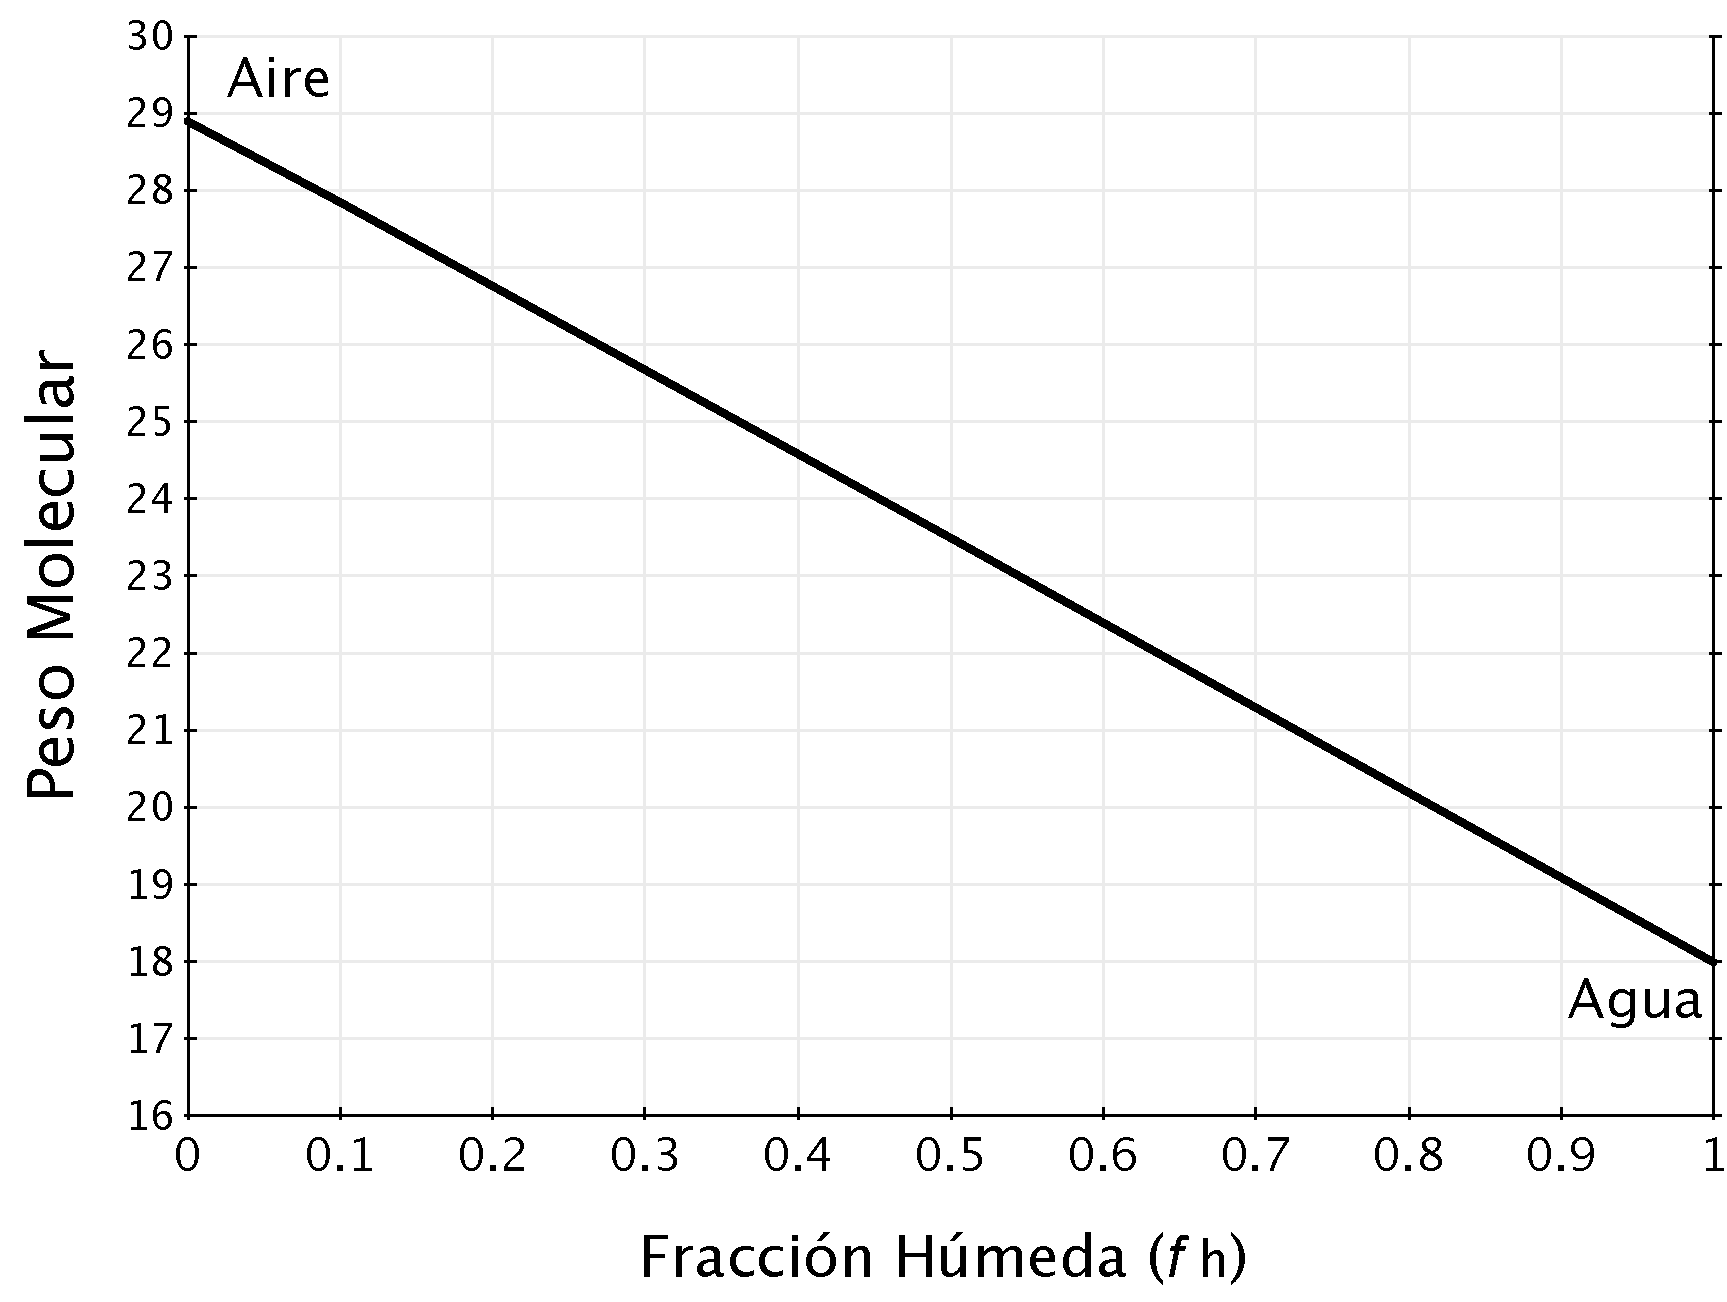
\includegraphics[width=0.70\textwidth]{FH.pdf}

\caption[Peso molecular aire-agua]{Cambio de la masa molecular promedio de la parcela con respecto a  la fracci\'on h\'umeda$f_H$ }
\label{fig_fh}
\end{center}
\end{figure}

\subsection{Flotabilidad de una parcela con humedad}\label{flopa}\index{flotacion@flotaci\'on}

La fuerza con la que es atra\'{\i}da por la gravedad una parcela de aire se puede estimar mediante:
\begin{equation}
F=V\rho g
\label{flot}
\end{equation}
Donde $V$ -- es el volumen, \gloss[word]{densidad} -- es la densidad del aire y $g$  --  es la aceleraci\'on de la gravedad. Substituyendo la  ecuaci\'on~\ref{dens} y ~\ref{pmh} en la ecuaci\'on~\ref{flot} tenemos:
\begin{equation}
F=\left[  (1-f_H)M_a + f_H M_{\ce{H2O}}\right] \frac{\textrm{PV}}{\textrm{RT}}g
\label{fb}
\end{equation}

\begin{figure}[htbp]
\begin{center}
\setlength{\unitlength}{1mm}
\begin{picture}(50,40)
\put (5,5){\line(2,1){7}} %Linea inf derecha
\put(12,8.5){\line(1,0){20}}% linea inf de atras
\put(12,8.5){\line(0,1){25}}
\thicklines
\put(5,30){\line(1,0){20}\line(2,1){7}} %Lineas superiores
\put(5,30){\line(2,1){7}}
\put(12,33.5){\line(1,0){20}} 
\put (5,5){\line(1,0){20}\line(2,1){7}} % Lineas Inferiores
\multiput(5,5)(20,0){2}{\line(0,1){25}}
\put(32,8.5){\line(0,1){25}}
% Flecha y texto izquierdo
%\put(3,19){\vector(0,1){11}}
%\put(3,15){\vector(0,-1){10}} % Flecha abajo
%\put(0,16){$dz$}
% Parte derecha
%\put(34,8){{\footnotesize $z$}}
%\put(34,19){{\footnotesize $\rho$}}
\put(14,16){{\footnotesize $F_g$}}
\put(18,15){\vector(0,-1){6}}
\put(19,22){{\footnotesize $F_b$}}
\put(18,21){\vector(0,1){6}}
%\put(34,32){\footnotesize $z+dz$}
% Parte inferior
%\put(9,1){{\scriptsize $P_b A$}}
%\put(16,0){\vector(0,1){5}}
\end{picture}
\caption{Fuerzas en una parcela de flotaci\'on ($F_b$) y atracci\'on por la gravedad ($F_g$).}
\label{fig_flo1t}
\end{center}
\end{figure}
El principio de Arqu\'{\i}medes nos dice que la fuerza de flotaci\'on ($F_b$) es igual al volumen desplazado, considerando que se desplaza aire seco ($f_H=0$), como se observa en la Figura~\ref{fig_flo1t}, entonces la ecuaci\'on~\ref{fb} quedar\'{\i}a: 
\begin{equation}
F_b=  M_a  \frac{\textrm{PV}}{\textrm{RT}}g
\label{fb1}
\end{equation}

Por otra parte la parcela con humedad ($f_H>0$) es atra\'{\i}da por la fuerza de gravedad ($F_g$) y ser\'{\i}a igual a:

\begin{equation}
F_g=\left[  (1-f_H)M_a + f_H M_{\ce{H2O}}\right] \frac{\textrm{PV}}{\textrm{RT}}g
\label{fg}
\end{equation}

Para las mismas condiciones de presi\'on (P) y temperatura (T),  y observando que el t\'ermino $M_a$ es mayor que $[(1-f_H)M_a + f_H M_{\ce{H2O}}]$ nos indica que $F_b$ es mayor que la fuerza de atracci\'on de la gravedad $F_g$, haciendo que la parcela con humedad, rodeada de aire seco, posea una resultante ascendente.

\subsection{Aceleraci\'on de una parcela con humedad}\label{acpa}
Se puede estimar la aceleraci\'on de una parcela inestable, de ah\'{\i} se puede estimar la velocidad en un tiempo dado. La aceleraci\'on (a) ascendente se le conoce como flotaci\'on (B).
\begin{figure}[htbp]
\begin{center}
\setlength{\unitlength}{1mm}
\begin{picture}(50,40)
\put (5,5){\line(2,1){7}} %Linea inf derecha
\put(12,8.5){\line(1,0){20}}% linea inf de atras
\put(12,8.5){\line(0,1){25}}
\thicklines
\put(5,30){\line(1,0){20}\line(2,1){7}} %Lineas superiores
\put(5,30){\line(2,1){7}}
\put(12,33.5){\line(1,0){20}} 
\put (5,5){\line(1,0){20}\line(2,1){7}} % Lineas Inferiores
\multiput(5,5)(20,0){2}{\line(0,1){25}}
\put(32,8.5){\line(0,1){25}}
% Flecha y texto izquierdo
\put(3,19){\vector(0,1){11}}
\put(3,15){\vector(0,-1){10}} % Flecha abajo
\put(0,16){$\mathrm{d}z$}
% Parte derecha
\put(34,8){{\footnotesize $z$}}
\put(13,15){{\footnotesize $\rho'gA\,\mathrm{d}z$}}
\put(34,19){{\footnotesize $\rho$}}
\put(16,13){\vector(0,-1){6}}
\put(17,35){{\footnotesize $P_s A$}}
\put(16,37){\vector(0,-1){6}}
\put(34,32){\footnotesize $z+\mathrm{d}z$}
% Parte inferior
\put(9,1){{\scriptsize $P_b A$}}
\put(16,0){\vector(0,1){5}}
\end{picture}
\caption{Fuerzas en una parcela con densidad diferente a los alrededores}
\label{fig_flot}
\end{center}
\end{figure}

Las fuerzas que act\'uan sobre la parcela, se muestran en la Fig.\ref{fig_flot}, la fuerza de flotaci\'on $F_b$ se representa como la fuerza ascendente ($P_bA$), la fuerza de la columna de aire ($F_s = P_sA$) y el peso de la parcela ($\rho'gA\,\mathrm{d}z$). Las cantidades asociadas a la parcela se identifican con el ap\'ostrofe (') y los par\'ametros ambientales no lo poseen.
\begin{equation}
\sum F= F_b +F_s+F_\textrm{peso} =P_bA-P_sA-\rho'gA\,\mathrm{d}z
\label{balance1}
\end{equation}

Las fuerzas de la ec.~\ref{balance1} no est\'an en equilibrio, as\'{\i} tenemos la necesidad de mantener la aceleraci\'on. Dividiendo ambos lados de la ecuaci\'on por la masa de la parcela ($\rho'V$), y que para el caso de la atm\'osfera terrestre $\mathrm{d}P/\mathrm{d}z= -\rho g$ tenemos:
\begin{equation}
\frac{\sum F}{\rho'V}= \frac{-\frac{P_s-P_b}{dz}-\rho'g}{\rho'}=\frac{-(-\rho g)-\rho'g}{\rho'}
\label{balance2}
\end{equation}
Considerando que se encuentra la parcela de aire a la misma temperatura del aire seco de los alrededores, sabiendo  que $\rho=PM/RT$y que  la aceleraci\'on (a)  $a=F/m$ :
\begin{equation}
a\equiv B=\frac{(\rho -\rho')g}{\rho'}= \frac{(M_a-M_w)g}{M_w}
\label{balance3}
\end{equation}

Sustituyendo la ecuaci\'on~\ref{pmh} en la ecuaci\'on~\ref{balance3} nos da que la aceleraci\'on por flotaci\'on (B) es:
\begin{equation}
B=\frac{(M_a-M_{\ce{H2O}})f_H }{M_a-(M_a-M_{\ce{H2O}})f_H} g
\label{bouyant}
\end{equation}
Al substituir los valores de $M_a$ y $M_{\ce{H2O}}$ , considerando que fuera  vapor de agua exclusivamante ($f_H=1$) la ecuaci\'on~\ref{bouyant} nos indica que la aceleraci\'on m\'axima de una parcela seria de  $6$ \metre/\square\second . La ecuaci\'on anterior nos indica que cualquier parcela que contenga vapor de agua va a ascender.

Para el caso cuando las temperaturas no son iguales,  donde $T_1$ es la temperatura del aire, $T_2$ es de la parcela tenemos:
\begin{equation}
B=\frac{\frac{T_2}{T_1}M_a-M_a+(M_a-M_{\ce{H2O}})f_H }{M_a-(M_a-M_{\ce{H2O}})f_H} g
\label{bouyant2}
\end{equation}
Para el caso de una parcela con humedad y m\'as caliente que los alrededores ($T_2>T_1$) la aceleraci\'on de la flotaci\'on ser\'a mayor que cuando las temperaturas son iguales ($T_2=T_1$). 

\section[Cin\'etica]{Cin\'etica Qu\'{\i}mica}
\label{cineq}

La cinética química es la rama de la química que se encarga de estudiar la velocidad de las reacciones químicas y los factores que inciden sobre ésta. Es decir, se ocupa de analizar cómo cambia la concentración de los reactivos y productos a lo largo del tiempo durante una reacción química.

La velocidad de una reacción química indica que tanto  los reactivos se convierten en productos. Esta velocidad se ve influenciada por diversos factores, como la concentración de los reactivos, la temperatura, la presión, el área de superficie de los reactivos, la presencia de catalizadores y la presencia de inhibidores.

La cinética química utiliza experimentos y métodos matemáticos para determinar la forma en que la velocidad de una reacción varía con respecto a los cambios en los factores mencionados anteriormente. A partir de estos estudios, se pueden obtener ecuaciones cinéticas que describen cómo la concentración de los reactivos y productos cambia en función del tiempo.

Existen diferentes tipos de reacciones químicas, y la cinética química permite clasificarlas en reacciones rápidas o lentas. Además, proporciona información sobre los mecanismos de reacción, que son las etapas o pasos individuales que ocurren durante una reacción química.

La cinética química es de gran importancia en diversas áreas, como la síntesis de productos químicos, la producción de energía, la industria farmacéutica y la investigación en ciencias ambientales. Comprender la velocidad de las reacciones químicas es fundamental para optimizar los procesos industriales, desarrollar nuevos medicamentos y comprender cómo los contaminantes afectan al medio ambiente.


\section{Velocidades de reacción}\index{velocidades@velocidades de reacción}\label{vreac}
Las velocidades de reacción se refieren a la rapidez con la que ocurre una reacción química en particular. Estas velocidades pueden variar ampliamente, desde reacciones muy rápidas que ocurren en fracciones de segundo hasta reacciones extremadamente lentas que pueden llevar días o incluso años para completarse.

La velocidad de una reacción química se determina midiendo cómo cambia la concentración de los reactivos o productos a lo largo del tiempo. Por lo general, se expresa como la cantidad de sustancia que se forma o se consume por unidad de tiempo.

Existen diferentes formas de expresar las velocidades de reacción. La más común es la velocidad promedio, que se calcula dividiendo el cambio en la concentración de un reactivo o producto entre un intervalo de tiempo determinado. Sin embargo, es importante tener en cuenta que la velocidad de una reacción puede cambiar a medida que los reactivos se consumen y los productos se forman, por lo que la velocidad instantánea, que se obtiene en un punto específico de la reacción, puede ser diferente a la velocidad promedio.

En resumen, las velocidades de reacción se refieren a la rapidez con la que ocurre una reacción química y se determinan mediante la medición de los cambios en la concentración de los reactivos o productos a lo largo del tiempo. La fotólisis es un tipo de reacción que implica la descomposición de sustancias mediante la absorción de energía radiante, como la luz. La luz actúa como un agente activador que proporciona la energía necesaria para romper los enlaces químicos y generar productos diferentes.

La reacciones en la fase gas se pueden clasificar dependiendo del n\'umero de reactivos involucrados as\'{\i} tenemos que las siguientes leyes de velocidad:
\begin{enumerate}
\item Reacciones de primer orden.

Una reacción de primer orden es una reacción química en la que la velocidad de reacción depende de la concentración de un solo reactivo elevado a la primera potencia. En otras palabras, la velocidad de la reacción es directamente proporcional a la concentración del reactivo.
	 \begin{equation*}
	\frac{\mathrm{d}\textrm[A]}{\mathrm{d}t}=-k[\textrm{A}]
	\end{equation*}
Donde $\mathrm{d}[A]/\mathrm{d}t$ representa la velocidad de la reacción, $k$ es la constante de velocidad y $[A]$ es la concentración del reactivo $A$. La constante de velocidad $k$ es una constante específica para una reacción dada y depende de la naturaleza de la reacción y de la temperatura.

La cinética de una reacción de primer orden implica que la velocidad de reacción disminuye a medida que la concentración del reactivo disminuye. Esto se debe a que hay menos moléculas de reactivo disponibles para reaccionar, lo que reduce las colisiones efectivas y, por lo tanto, disminuye la velocidad de la reacción.

Un ejemplo común de una reacción de primer orden es la descomposición radioactiva. En este caso, la concentración de un isótopo radiactivo disminuye con el tiempo debido a su desintegración. La velocidad de desintegración de un isótopo radiactivo es proporcional a la concentración del isótopo presente, y se expresa mediante una constante de velocidad específica para ese isótopo. Otros ejemplos los tenemos con:
 \ce{A -> B +C}\index{reaccion@reacci\'on!unimolecular}
	\begin{description}
		\item[a) Fot\'olisis]  \ce{NO2 + h{\nu} -> NO + O {\cdot}}
		\item[b) T\'ermicas] \ce{CH3COONO3 -> CH3-CO3 + NO2}
	\end{description}
Integrando la ecuaci\'on tenemos:
	\begin{equation*}
	\ln \textrm{A} = -kt
	\end{equation*}
	donde las unidades de $k$ son $s^{-1}$ y de A  son moléculas/cm$^3$
	
En resumen, una reacción de primer orden es aquella en la que la velocidad de reacción es directamente proporcional a la concentración de un solo reactivo elevado a la primera potencia. Estas reacciones se describen mediante una expresión matemática que muestra cómo la velocidad de reacción varía con la concentración del reactivo. En el caso de una reacción atmosférica, la descomposición del ozono puede considerarse como una reacción de primer orden, donde la velocidad de descomposición está determinada principalmente por la concentración de ozono presente en la atmósfera.

\item Reacciones de Segundo Orden  \ce{A + B -> C + D}\\\index{reaccion@reacci\'on!bimolecular}
Las reacciones de segundo orden son un tipo de reacción química en la cual la velocidad de reacción depende de la concentración de dos reactivos diferentes. Es decir, la velocidad de reacción es proporcional al producto de las concentraciones de ambos reactivos elevadas a la primera potencia. Matemáticamente, se representa mediante una ecuación de segundo orden.

En el contexto de la química atmosférica, un ejemplo común de una reacción de segundo orden es la reacción entre los óxidos de nitrógeno (NOx) y el ozono (\ce{O3}). Estos compuestos son precursores de la formación de smog fotoquímico y tienen un impacto significativo en la calidad del aire.
\reaction{O3 + NO -> NO2 + O2}
La reacción entre los óxidos de nitrógeno y el ozono puede describirse como una reacción de segundo orden, donde la velocidad de reacción depende de la concentración de ambos reactivos. La ecuación cinética general para una reacción de segundo orden se expresa de la siguiente manera:
 \begin{equation*}
\ce{Rapidez = - k[NOx][O3]}
 \end{equation*}
Donde ``Rapidez'' representa la velocidad de reacción, $k$ es la constante de velocidad y [NOx] y [\ce{O3}] son las concentraciones de los reactivos óxidos de nitrógeno y ozono, respectivamente.

En este caso, la velocidad de reacción es proporcional al producto de las concentraciones de óxidos de nitrógeno y ozono. A medida que aumentan las concentraciones de ambos reactivos, la velocidad de reacción también aumenta. Sin embargo, si la concentración de uno de los reactivos disminuye, la velocidad de reacción disminuirá en consecuencia.

La reacción de segundo orden entre los óxidos de nitrógeno y el ozono es importante en la química atmosférica, ya que contribuye a la formación de oxidantes fotoquímicos, como el dióxido de nitrógeno (\ce{NO2}), que puede tener efectos adversos en la salud humana y en el  ambiente.

 \begin{equation*}
	-\frac{\mathrm{d}[\textrm{A}]}{\mathrm{d}t}=-\frac{\mathrm{d}[\textrm{B}]}{\mathrm{d}t}=\frac{\mathrm{d}[\textrm{C}]}{\mathrm{d}t}=k[\textrm{A}][\textrm{B}]
	\end{equation*}
	las unidades de k son {\centi\cubic\metre}/{molec$\cdot $\second}
	
En resumen, las reacciones de segundo orden son aquellas en las que la velocidad de reacción depende de la concentración de dos reactivos diferentes. En el caso de la química atmosférica, un ejemplo de una reacción de segundo orden es la reacción entre los óxidos de nitrógeno y el ozono. La velocidad de reacción está determinada por el producto de las concentraciones de ambos reactivos y desempeña un papel importante en la formación de contaminantes atmosféricos como el smog fotoquímico.

\item Termoleculares \ce{A + B + C -> D  + E +\ldots}\\\index{reaccion@reacci\'on!termolecular}
Las reacciones termoleculares son un tipo de reacción química en la que tres o más moléculas colisionan y se combinan para formar productos. Estas reacciones son bastante comunes en la química atmosférica y desempeñan un papel importante en la formación y degradación de diferentes compuestos presentes en la atmósfera.

En el contexto de la química atmosférica, un ejemplo de una reacción termolecular es la formación de ozono (\ce{O3}) a partir del oxígeno molecular (\ce{O2}). Esta reacción ocurre en la estratosfera, donde la radiación ultravioleta proveniente del sol desencadena una serie de procesos fotoquímicos.

La formación de ozono se puede describir mediante la siguiente reacción termolecular:

\reaction{O2 + O2 + M ->  O3 + M}

En esta reacción, dos moléculas de oxígeno (\ce{O2}) colisionan con una molécula inerte (representada como M) y se combinan para formar una molécula de ozono (\ce{O3}) y otra molécula inerte.

En la atmósfera superior las reacciones termoleculares son más comunes  ahí las densidades de moléculas son más bajas y,  la probabilidad de colisiones múltiples aumentan. Estas reacciones juegan un papel importante en la química atmosférica, ya que contribuyen a la formación y degradación de diferentes especies químicas.

Hay que considerar que las reacciones termoleculares pueden ser altamente dependientes de la energía y la temperatura. La energía necesaria para superar la barrera de activación y permitir que las moléculas colisionen de manera efectiva es proporcionada por la radiación solar en el caso de la atmósfera terrestre.

Así tenemos que las reacciones termoleculares involucran la colisión de tres o más moléculas para formar productos. Un ejemplo destacado es la formación de ozono a partir del oxígeno molecular. Estas reacciones son importantes para comprender los procesos fotoquímicos y la formación de diferentes compuestos atmosféricos en la estratosfera y otras regiones de la atmósfera.

\reaction{O2 + O + M -> O3 + M}

 \begin{equation*} -\frac{\mathrm{d}[\textrm{A}]}{\mathrm{d}t}=k[\textrm{A}][\textrm{B}][\textrm{C}]
 \end{equation*}
 
 \item Heterog\'eneas (entre fases): Gobernadas por la difusi\'on molecular. La velocidad de colisi\'on del \'atomo B en una superficie por unidad de \'area =$\bar{c}$/4[B]. \index{reaccion@reacci\'on!heterogenea}
\begin{equation*}
-\frac{\mathrm{d}[\textrm{B}]}{\mathrm{d}t}=\frac{\bar{c}}{4}[\textrm{B}]\alpha A
\end{equation*}
 donde $\bar{c}$ es la velocidad molecular promedio \begin{equation}
\bar{c}=\left(\frac{8kT}{\pi M}\right)^{0.5}
\end{equation}
$A$ es el \'area de superficie y $\alpha$ es el coeficiente de adhesi\'on
\end{enumerate}

\section{Tiempo de vida media}\index{vida@vida media}\index{tiempo!de vida media}\label{TVDM}
Definiremos el tiempo de vida media de un reactivo como el tiempo necesario para que haya reaccionado la mitad de su concentración inicial

En el caso de una reacción de primer orden, cuya ecuación de velocidad sabemos que es: 

\begin{equation*}
\nu =k\cdot [A]
\end{equation*}

Entonces, según la definición de  $t_{1/2}$ , tenemos que:

\begin{equation*}
t=t_{1/2} \Longrightarrow  [A]=\frac{[A]_0}{2}
\end{equation*}

Usando la fórmula logarítmica para las reacciones de primer orden:
\begin{equation*}
\ln[A]=\ln[A]_0-k\cdot t
\end{equation*}
tendremos que: 

$$\ln\frac{[A]_0}{2}=\ln[A]_0-k\cdot t_{1/2}$$

por lo que:

$$\ln[A]_0-\ln2-\ln[A]_0=-k\cdot t_{1/2}$$

y nos queda que:

$$t_{1/2}=\frac{-\ln2}{-k}=\frac{\ln2}{k}$$

De esta expresión, vemos que el tiempo de vida media es, en este caso, independiente de la concentración inicial. Por otra parte, se evidencia que la constante de velocidad específica tiene dimensiones de tiempo$^{-1}$y también es independiente de la concentración inicial.

\section{Tiempo de residencia}\index{tiempo!de residencia}\label{tdres}
Los productos químicos se inyectan continuamente en la atmósfera desde fuentes naturales y antrópicas\index{antrópica}, y también se producen por reacciones químicas en el aire. Sin embargo, la composición química general de la atmósfera no cambia mucho en períodos de tiempo relativamente cortos (aunque, como veremos, hay excepciones importantes). Esto se debe a que existen sumideros que eliminan trazas de sustancias químicas de la atmósfera aproximadamente a la misma velocidad con la que se inyectan (y/o se producen dentro) de la atmósfera, de modo que la mayoría de las sustancias químicas en el aire existen en condiciones más o menos estables.s

Un parámetro importante relacionado con una sustancia química en condiciones de estado estacionario es su tiempo de residencia o vida útil (\gloss[word]{tresid}) en la atmósfera, que se define como:
\begin{equation*}
\tau=\frac{M}{F}
\end{equation*}
donde $M$ es la cantidad de sustancia química en la atmósfera y $F$ la salida (es decir, tasa de eliminación más tasa de destrucción) de la sustancia química de la atmósfera. Si $M$ y $F$ cambian con el tiempo
\begin{equation*}
\tau_t=\frac{M_t}{F_t}
\end{equation*}
donde el subíndice $t$ indica el valor en el momento t. Podemos definir, de manera análoga, el tiempo de residencia en términos del influjo (es decir, tasa de entrada más tasa de producción) de una sustancia química a la atmósfera.

\begin{table}[!hb]
\caption{Tiempo de residencia de gases atmosféricos}
\begin{center}
\begin{small}
\begin{tabular}{|l|c|}\hline
\textbf{Gas}                           &\textbf{Tiempo de residencia} \\ \hline
Nitrógeno (\ce{N2})              &  $1.6\times10^7$ a \\
Oxígeno (\ce{O2})	            &3,000 -- 10,000 a \\
Dióxido de Carbono  (\ce{CO2})& 3 -- 4 a \\
Metano (\ce{CH4})                &    9 a  \\
Ozono	 (\ce{O3})              &      100 dia \\
Monóxido de carbono (CO)   &     $\sim  60$ dia \\
Formaldehído	 (\ce{CHOH})& 5 -- 10 dia \\
Dióxido de Nitrógeno (\ce{NO2})&0.5 -- 2 dia\\ \hline
\end{tabular}
\end{small}
\end{center}
\label{tresidencia}
\end{table}%

\begin{figure}[htbp]
\begin{center}
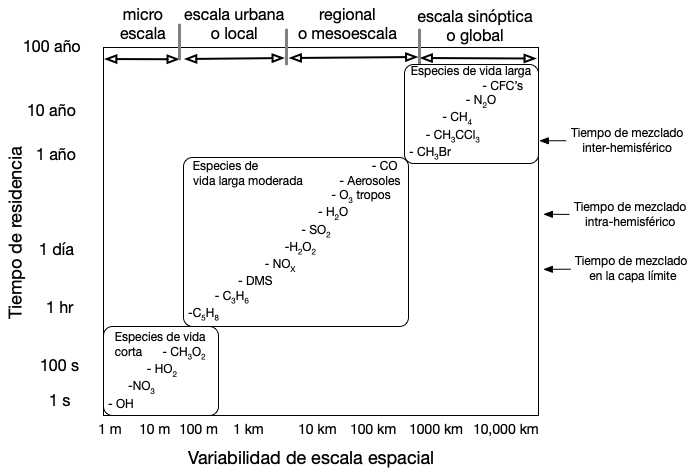
\includegraphics[width=0.95\textwidth]{tiempo_residencia.png}

\caption[Tiempos de residencia]{Tiempos de residencia de gases en la atmósfera.}
\label{fig_tresidencia}
\end{center}
\end{figure}
Si una especie química tiene un tiempo de residencia muy corto (o muy largo) en la atmósfera, generalmente se producirán variaciones significativas en la concentración de la especie en escalas espaciales muy cortas (o muy grandes) (Fig.~\ref{fig_tresidencia}). Las especies con tiempos de residencia cortos estarán presentes en altas concentraciones cerca de fuentes localizadas y en bajas concentraciones muy alejadas de sus fuentes.

\section{Fotoqu\'{\i}mica}\index{fotoquimica@fotoqu\'{\i}mica}\label{fqm}

La contaminaci\'on en las ciudades se da principalmente por la conversi\'on de los contaminantes primarios a contaminantes secundarios mediante la interacci\'on con la luz solar. Estos contaminantes se caracterizan principalmente por su alto nivel de oxidaci\'on que afectan los materiales, plantas e irritan ojos y garganta. As\'{\i}mismo influyen en la disminuci\'on de la visibilidad y generaci\'on de olores.

No toda la luz participa en las reacciones, s\'olo la luz que es absorbida puede producir un cambio fotoqu\'{\i}mico, as\'{\i} tenemos que dependiendo de la longitud de onda (\gloss[word]{londa}) se pueden producir un efecto
\begin{enumerate}
\item El lejano IR, microondas influyen en la rotaci\'on de las mol\'eculas.\index{microondas}
\item El infrarrojo en la vibraci\'on
\item La luz visible y ultravioleta en niveles de electrones.
\end{enumerate}

La fotodisociaci\'on\index{fotodisociacion@fotodisociaci\'on} es un proceso en dos pasos el primero la absorci\'on de un fot\'on ($h\nu$)\index{foton@fot\'on} (donde  \gloss[word]{hplank}  es la contante de Planck)\index{constante!Planck} que conduce a un estado exitado.

 \begin{equation*}
\ce{A + h{\nu}    -> A^* } \end{equation*}
posteriormente se produce la disociaci\'on de A$^*$ en dos productos tales como:
\reaction*{A^* -> B + C}
 

\section{Visibilidad}\index{visibilidad}\label{vis2}

La visibilidad se reduce por la absorción y esparcimiento\index{esparcimiento} de la luz en materiales líquidos y sólidos suspendidos en el aire. Para la luz visible (longitud de onda $\lambda = 0.38$ a $0.70\ \micro\metre$), las partículas con diámetros entre $0.1$ y $1\ \micro\metre$ son particularmente efectivas en la dispersión lumínica, fenómeno que además tiene implicaciones en la salud respiratoria.

\subsection{Mecanismos de dispersión}\label{mddis}
\begin{itemize}
    \item \textbf{Dispersión Rayleigh} ($r \ll \lambda$):
    \begin{itemize}
        \item Dominante en moléculas gaseosas ($d \sim 0.001\ \micro\metre$)
        \item Dependencia espectral $\propto \lambda^{-4}$ (explica el color del cielo)
    \end{itemize}
    
    \item \textbf{Dispersión de Mie}\index{Mie@\textbf{Mie}!esparcimiento} ($r \sim \lambda$):
    \begin{itemize}
        \item Máxima eficiencia para $\lambda = 0.52\ \micro\metre$ (verde-amarillo)
        \item Direccionalidad preferencial hacia adelante (factor de asimetría $g \geq 0.7$)
    \end{itemize}
    
    \item \textbf{Difusión no selectiva} ($r > \lambda$):
    \begin{itemize}
        \item Dominada por partículas gruesas (> $1\ \micro\metre$)
        \item Escasamente dependiente de la longitud de onda
    \end{itemize}
\end{itemize}

La visibilidad se reduce por absorci\'on y esparcimiento de la luz de  materiales l\'{\i}quido y s\'olidos arrastrados por el aire. Los gases que afectan la visibilidad en el aire son el bi\'oxido de azufre (\ce{SO2}), el mon\'oxido de nitr\'ogeno (NO) y el vapor de agua. (\ce{H2O}). En el aire limpio se puede ver hasta una distancia de 150 millas y el humo llega a reducir la visibilidad de 1 a 3 millas. Una concentraci\'on de 2,000 part/cm$^3$ se polvo puede ocultar monta\~nas y 100,000 part/cm$^3$ reducen la visibilidad a 1 milla. Concentraciones de \ce{NO2} de 8 a 10 ppm reducen la visibilidad a 1 milla.

Consid\'erese un objeto iluminado por un rayo de intensidad ($I$), a una distancia $x$ del observador
\begin{equation}
\mathrm{d}I=-\sigma I\, \mathrm{d}x
\end{equation}
donde \gloss[word]{extincion} es el coeficiente de extinci\'on,\index{coeficiente!extincion@extinci\'on} $\mathrm{d}x$ es la distancia recorrida, $\mathrm{d}I$ es la reducci\'on de la intensidad por la absorci\'on y dispersi\'on e $I_0$ es la intensidad inicial. Integrando desde 0 a $d$ tenemos
\begin{equation}
I =I_0 e^{-\sigma d}
\end{equation}
$\sigma$ incluye efectos de absorci\'on y dispersi\'on de mol\'eculas de gas y aerosoles.

\begin{equation}
I = I_0 e^{-(\alpha + s)d} \quad \text{(Ley de Beer-Lambert extendida)}
\end{equation}
donde $\alpha$ es el coeficiente de absorci\'on\index{coeficiente!absorcion@absorci\'on} y $s$ es el coeficiente de esparcimiento.\index{coeficiente!esparcimiento}

La atenuaci\'on de la luz producida en la atm\'osfera por dipesi\'on se deben a par\'{\i}culas de tama\~no comparable a la longitud de onda (\gloss[word]{londa}) de la luz incidente. Esto es el esparcimiento de \gloss[Word]{mie}\index{Mie@\textbf{Mie}!esparcimiento} y es el fen\'omeno responsable de la reducci\'on de la visibilidad. En el esparcimiento de Mie, se genera m\'as esparcimiento hacia delante que en cualquier otra direcci\'on. Al aumentar el tama\~no de la part\'{\i}cula, el esparcimiento hacia delante tambi\'en aumenta.


La f\'ormula de dispersi\'on de Mie (S) es la siguiente:
\begin{equation}
S = NK\pi r^2 \quad \text{(Eficiencia de dispersión)}
\end{equation}
$N$ Densidad numérica  de part\'iculas de radio $r$ por unidad de volumen [cm$^{-3}$]. $K$ razón de eficiencia (${Q_{sca}}/{4}$ para esferas dieléctricas) y
$r$: radio de la partícula [$\micro\metre$]

La longitud de onda de la luz del Sol se encuentra entre 0.4 a 0.8\micro\metre\,  con un m\'aximo a 0.52\micro\metre\, por lo que part\'{\i}culas de 0.1 a 1{\micro\metre} son responsables de la disminuci\'on de la visibilidad. Part\'{\i}culas de tama\~no similar invaden los pulmones y afectan a la salud.

%\newpage
\begin{exercises}
Conteste con verdadero o falso, o complete las siguientes preguntas:

\exer Todas las reacciones qu\'{\i}micas ocurren  a  la misma velocidad\dotfill (\hskip.12in)\\
\exer La velocidad qu\'{\i}mica se define como el tiempo que tardan los productos en convertirse en reactivos.\dotfill(\hskip.12in)\\
\exer La teor\'{\i}a de las colisiones dice que todas las colisiones producen reacci\'on.\dotfill(\hskip.12in)\\
\exer Especie intermedia que s\'olo existe durante una fracci\'on de segundo y puede dar lugar a los productos o a reactivos es el complejo activado.\dotfill(\hskip.12in)\\
\exer Barrera de energ\'{\i}a que separa el estado de los reactivos y el estado de los produc\-tos es la energ\'{\i}a de activaci\'on \dotfill (\hskip.12in)
\exer Una neutralizaci\'on es aquella reacci\'on en donde se combina un \'acido con una base\dotfill (\hskip.12in)
\exer Escriba las expresiones de las constantes de equilibrio (kc) para las siguientes reacciones:
\subexer \ce{N2 + 3H2(g) ->  2NH3(g)}
\subexer \ce{N2O + 1/2O2 -> 2NO}
\subexer \ce{4NH3 + 3O2 -> 2N2 + 6H2O}
\subexer \ce{H2 + I2 -> 2HI}
\exer Si la constante de equilibrio $Kc$ para la reacci\'on\\ \vskip 3pt \ce{A(g) + 2B(g) <=> G(g)+ 3H(g)} es 2.1$\times10^{-3}$,\\ \vskip 3pt ?`Qu\'e concentraci\'on de H(g) se tiene en el equilibrio con 0.1 M de A(g), 0.25 de B(g) y 0.02M de G(g)
\exer Si la constante de equilibrio (kp)  para la reacci\'on\\\vskip 3pt\ce{2SO2(g) + O2(g) <=> 2SO3(g)} a 820$^\circ$C es 5.18. \\\vskip 3pt?`Cu\'al es la presi\'on parcial de \ce{SO3(g)} que estar\'{\i}a en equilibrio con 0.25 atm de \ce{SO2(g)} y 0.705 atm de \ce{O2(g)}
\exer Mencione tres factores que influyen en la velocidad de reacci\'on.\\
:\hrulefill ,\hrulefill y \hrulefill .
\exer  ?`C\'omo debe ser el valor de la constante de equilibrio ( $K_{eq}$ ) con respecto al uno para que el equilibrio se desplace hacia los productos?\hrulefill
\exer Si un sistema en equilibrio sufre una alteraci\'on el sistema responder\'a de tal forma que compense dicha alteraci\'on es el principio de:\hrulefill
\exer Una soluci\'on de un \'acido y su base conjugada forman una soluci\'on tam\-p\'on o Buffer\dotfill(\hskip.12in)\\
\exer Un \'acido es un donador de :\hrulefill
\exer En la siguiente reacci\'on se\~nale qu\'e compuestos se comportan como \'acido y cu\'ales como base \ce{HCl + H2O ->  H3O^+ + Cl^-}
\exer Un compuesto que puede reaccionar tanto como \'acido o como base se le conoce como:\hrulefill
\exer Llene los espacios en blanco:\\
\begin{tabular}{l|c|c|c|c}
Sustancia & $[H^+]$ & $pH$ & $pOH$ & [OH]\\ \hline
Leche de vaca &    & $6.6$ &$7.4$ &  \\
\hline Jugo de lim\'on & &$2$ & &$1\times10^{-12}$ \\
\hline 
\end{tabular}
\exer A partir de la siguiente reacci\'on:\\\vskip 3pt \ce{2HNO3 + Mg(OH)2 <=> Mg(NO3)2 + 2H2O}\\ \vskip 3pt ?`Qu\'e cantidad de \'acido n\'{\i}trico \ce{(HNO3)} puede reaccionar con 200 g de hidr\'oxido de magnesio \ce{(Mg(OH)2)}. 

\exer ?`Qu\'e significa la $p$ en el t\'ermino de $pH$:
\hrulefill

\exer Explique cómo los tres tipos de dispersión (Rayleigh, Mie y no selectiva) afectan la visibilidad en función del tamaño de partícula y la longitud de onda de la luz. Incluya un ejemplo de fenómeno atmosférico asociado a cada mecanismo.

\exer Utilizando la fórmula de Koschmieder(\ref{fKoschmieder}): 
\begin{equation*}
V=\frac{3.912}{\beta_{ext}}  \quad [\kilo\metre]
\end{equation*}
Calcule la visibilidad horizontal en los siguientes casos:
\begin{enumerate}
\item En una zona urbana con $\beta_{ext}=200 $Mm$^{-1}$.
\item Durante una niebla densa donde $\beta_{ext}=39,000 $Mm$^{-1}$.
\item Interprete qué sucede si la humedad relativa supera el 70\% en el valor de $\beta_{ext}$.
\end{enumerate}

\exer ?`Por qué las partículas menores a (\ce{PM_{2.5}}) son más críticas que las \ce{PM_{10}} para la visibilidad y la salud humana? Relacione su respuesta con:
\begin{enumerate}
\item El mecanismo de dispersión de Mie.
\item La capacidad de penetración en el sistema respiratorio.
\item La evolución histórica de las normas de calidad del aire (\ce{PST -> PM_{10} -> PM_{2.5}}). 
\end{enumerate}

\end{exercises}

%\begin{chapreferences}{Fisicoquimica de la Atmosfera}
%\bibitem[Cas86]{castellan}
%Gilbert~W. Castellan.
%\newblock {\em Fisicoqu\'{\i}mica}.
%\newblock Fondo de Educativo Interamericano, M\'exico, D.F., 1986.
%
%\bibitem[MP84]{maron}
%Samuel~H. Maron and Carl~F. Prutton.
%\newblock {\em Fundamentos de Fisicoqu\'{\i}mica}.
%\newblock Editorial LIMUSA, {M\'exico, D.F.}, 1984.
%\newblock decimocuarta reimpresi\'on.
% \end{chapreferences}
